%! Author = loreb
%! Date = 31/10/2023

\documentclass{article}

% Language setting
% Replace `english' with e.g. `spanish' to change the document language
\usepackage[italian]{babel}

% Set page size and margins
% Replace `letterpaper' with `a4paper' for UK/EU standard size
\usepackage[letterpaper,top=2cm,bottom=2cm,left=3cm,right=3cm,marginparwidth=1.75cm]{geometry}

% Useful packages
\usepackage{amsmath}
\usepackage{amsfonts}
\usepackage{graphicx}
\usepackage{mathrsfs}
\usepackage[colorlinks=true, allcolors=blue]{hyperref}
\usepackage{subcaption}
\usepackage{float}

\usepackage[font=small,labelfont=bf]{caption}

\title{K-means and Mixed-Integer Quadratic Programming}
\author{Lorenzo Baiardi \& Thomas Del Moro}

\begin{document}
    \maketitle
    \begin{abstract}
        K-means è uno degli algoritmi più conosciuti e utilizzati per molti problemi di clustering. In questo lavoro analizziamo un approccio innovativo del k-means, basato sulla tecnica di Mixed-Integer Quadratic Programming (MIQP). Attraverso l'utilizzo di dataset sintetici e real-world valutiamo le performance di questa tecnica, in modo da comprenderne le
        eventuali potenzialità e criticità in ambito empirico.
    \end{abstract}


    \section{Introduzione}

    Questo lavoro consiste nell'analisi sperimentale dell'approccio MIQP relativamente all'algoritmo K-means. In particolare i nostri studi si concentrano su un confronto tra tale versione con quella originale, sulla base di vari aspetti quali la l'andamento della funzione obiettivo e il tempo di esecuzione al variare dei parametri del dataset utilizzato.

    \subsection{K-Means}

    Consideriamo un dataset numerico $D=\{x_i \in \mathbb{R}^{N}, i=1,\dots,n$. Applicare l'algoritmo k-means significa partizionare gli esempi $x_i$ in $K$ cluster, con $K$ fissato, in modo da minimizzare la somma delle distanze euclidee al quadrato tra ogni elemento del dataset e il centroide del cluster al quale è assegnato.
    Formalmente il problema è dato da
    \begin{equation}
        \min_{\begin{subarray}{c}
                  \delta \in \{0, 1\}^{n \times K}\\
                  z \in \mathbb{R}^{K \times N}
        \end{subarray}}
        \frac{1}{2} \sum_{i=1}^{n} \sum_{k=1}^{K} \delta_{ik} \|x_i-z_k\|^2
        \label{eq:kmeans}
    \end{equation}
    dove $\delta_{ik}$ sono le variabili indicatrici dell'associazione tra il punto $x_i$ e il cluster $k$, mentre le $z_k$ indentificano il centroide del cluster $k$.\\
    A questo problema sono poi stati aggiunti dei vincoli di appartenenza, per cui ogni punto può essere associato a un solo cluster e ad ogni cluster devono essere associati almeno $C$ elementi. Dunque il problema diventa
    \begin{equation}
        \begin{aligned}
            \min_{\substack{
                \delta \in \{0, 1\}^{n \times K}\\
                z \in \mathbb{R}^{K \times N}}} &
            \frac{1}{2} \sum_{i=1}^{n} \sum_{k=1}^{K} \delta_{ik} \|x_i-z_k\|^2 \\
            \text{t.c.} \quad &
            \begin{aligned}
                & \sum_{k=1}^{K} \delta_{ik} = 1 \quad \text{for $i=1,\dots,n$}\\
                & \sum_{i=1}^{n} \delta_{ik} \geq C_k \quad \text{for $k=1,\dots,K$}
            \end{aligned}
        \end{aligned}
        \label{eq:constrained_kmeans}
    \end{equation}

    In questa formulazione l'algoritmo viene inizializzato con dei centroidi casuali, dopodiché ripete iterativamente i seguenti due step:
    \begin{itemize}
        \item \textbf{Assegnazione}: ogni elemento $x_i$ viene assegnato al cluster $k$ il cui centroide è più vicino a $x_i$ tra tutti i centroidi
        \[\delta^{t+1} \in \arg \min_{\delta \in \{0,1\}^n\times \K} \frac{1}{2} \sum_{i=1}^{n} \sum_{k=1}^{K} \delta_{ik} \|x_i-z_k^{t}\|^2\]
        \item \textbf{Aggiornamento}: tutti i centroidi vengono aggiornati come la media dei punti assegnati al loro cluster
        \[z^{t+1} \in \arg \min_{z} \frac{1}{2} \sum_{i=1}^{n} \sum_{k=1}^{K} \delta_{ik}^{t+1} \|x_i-z_k\|^2\]
        in particolare si può verificare che vale la soluzione calcolabile in forma chiusa
        \[z_k^{t+1} = \frac{\sum_{i=1}^{n} \delta_{ik}^{t+1} x_i}{\sum_{i=1}^{n} \delta_{ik}^{t+1}}\]
    \end{itemize}

    \subsection{MIQP K-Means}
    Il MIQP (acronimo di Mixed-Integer Quadratic Programming) è una combinazione di Quadratic Programming e Mixed-Integer Linear Programming, più in particolare è una classe di problemi di ottimizzazione che consiste nel minimizzare una funzione quadratica di variabili continue soggette a vincoli lineari, ma alcune delle variabili sono anche soggette a vincoli di interezza.\\
    Molti problemi di ottimizzazione possono essere riformulati come MIQP e risolti attraverso l'utilizzo di solver (es. Gurobi) che oggi sono capaci di gestire un gran numero di variabili intere e trovare l'ottimo globale del problema.\\
    Nel nostro caso, quindi, il problema di clustering può essere riformulato in modo da garantire, tramite l'utilizzo di un solver, il raggiungimento dell'ottimo globale; in contrasto con la versione classica di K-Means che è soggetta allo stazionamento in minimi locali.\\
    Il problema~\ref{eq:constrained_kmeans} può dunque essere riformulato come
    \begin{equation}
        \begin{aligned}
            \min_{\substack{
                \delta \in \{0, 1\}^{n \times K}\\
                z \in \mathbb{R}^{K \times N} \\
                s \in \mathbb{R}^{N \times n \times K}}} &
            \frac{1}{2} \sum_{i=1}^{n} \sum_{k=1}^{K} \|s_{ik}\|^2 \\
            \text{t.c.} \quad &
            \begin{aligned}
                & \sum_{k=1}^{K} \delta_{ik} = 1 \quad \text{for $i=1,\dots,n$} \\
                & \sum_{i=1}^{n} \delta_{ik} \geq C_k \quad \text{for $k=1,\dots,K$} \\
                & -M(1-\delta_{ik}) + (x_{ij}-z_{kj}) \leq s_{jik} \leq M(1-\delta_{ik}) + (x_{ij}-z_{kj}) \quad \text{for all $i, j, k$}
            \end{aligned}
        \end{aligned}
        \label{eq:MIQkmeans}
    \end{equation}
    dove $M$ è un valore sufficientemente grande da garantire che:
    \begin{itemize}
        \item se $\delta_{ik} = 0$ allora $s_{jik}$ sia uguale alla distanza tra $x_{ij}$ e $z_{kj}$.
        \item se $\delta_{ik} = 1$ allora $s_{jik}$ sia libero e quindi settato a 0.
    \end{itemize}

    \section{Implementazione}
    Per l'algoritmo K-Means, una volta inizializzati i centroidi, viene eseguito lo step di assegnazione degli indicatori, utilizzando l'ottimizzazione del solver Gurobi. Per l'aggiornamento dei centroidi invece si è utilizzato il calcolo in forma chiusa mostrato sopra.\\
    La versione MIQP invece si basa interamente sull'ottimizzazione del solver Gurobi. In questo caso era necessario impostare un valore ragionevole di time limit, per evitare esecuzioni eccessivamente lunghe. Notiamo che la costante $M$ utilizzata nei vincoli deve essere impostata al valore più piccolo possibile che non introduca vincoli di box, in modo da migliorare l'efficienza dell'algoritmo.\\

    \section{Esperimenti e Risultati}
    Entrambi gli algoritmi sono stati testati su dataset sintetici e real-world osservando principalmente il valore della funzione obiettivo e il tempo di esecuzione. In particolare sono stati confrontati tali risultati al variare dei fattori $n$, $N$, e $K$, in modo da comprendere le eventuali criticità delle due formulazioni del problema.\\
    \subsection{Test visuali}
    Prima di tutto sono stati eseguiti alcuni test visuali per analizzare il comportamento dei due algoritmi. Per farlo, è stato utilizzato un algoritmo di PCA, che ha permesso di costruire uno scatterplot in due dimensioni dei dati clusterizzati. In Figura \ref{fig:1} sono mostrati alcuni esempi di clustering ottenuti con la versione MIQP di K-Means eseguito su dataset relativamente piccoli generati artificialmente.
    \begin{figure}[h]
     \centering
     \begin{subfigure}[b]{0.32\linewidth}
         \centering
         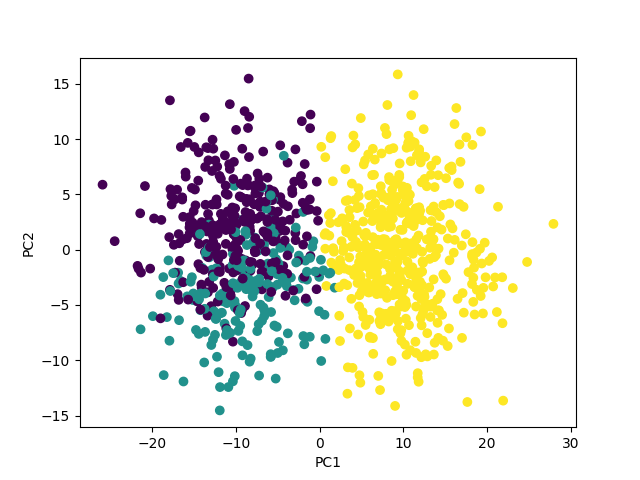
\includegraphics[width=\linewidth]{../results/plots/scatter_k3}
         \caption{3 cluster}
     \end{subfigure}
     \hfill
     \begin{subfigure}[b]{0.32\linewidth}
         \centering
         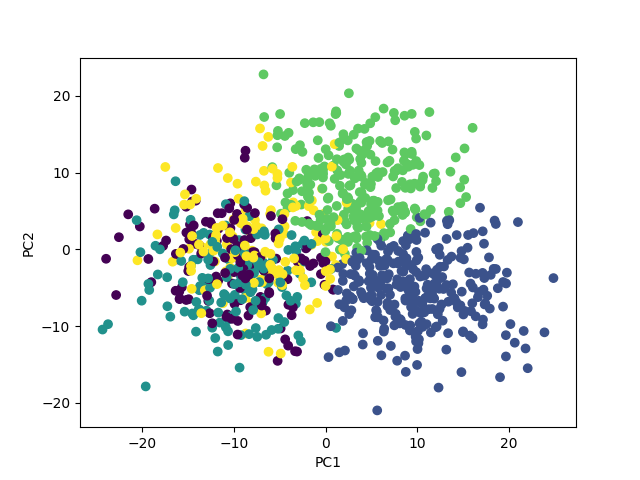
\includegraphics[width=\linewidth]{../results/plots/scatter_k5}
         \caption{5 cluster}
     \end{subfigure}
     \begin{subfigure}[b]{0.32\linewidth}
         \centering
         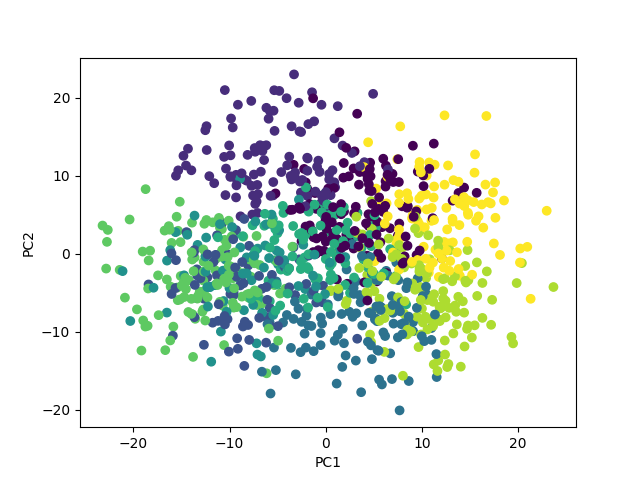
\includegraphics[width=\linewidth]{../results/plots/scatter_k7}
         \caption{7 cluster}
     \end{subfigure}
     \caption{Scatterplot dei dati clusterizzati con MIQP K-Means}
     \label{fig:1}
    \end{figure}
    In tutti i casi è stato impostato un time-limit per la versione MIQP per ottenere i risultati in tempi ragionevoli. Ciò ovviamente porta a ottenere una soluzione sub-ottima anche con questa versione del'algoritmo. Tuttavia, poiché il funzionamento degli algoritmi è diverso, anche tale soluzione sub-ottima sarà probabilmente diversa. Come è possibile notare in Figura \ref{fig:2} il K-Means costruisce sempre cluster di forma globulare. Diversamente, la versione MIQP (con time-limit) può essere interrotta prima di aver assegnato ogni punto al cluster più vicino. Sarà più probabile, quindi, avere dei cluster più omogenei in cui però alcuni punti singolari potranno essere etichettati in modo evidentemente errato.
    \begin{figure}[h]
     \centering
     \begin{subfigure}[b]{0.49\linewidth}
         \centering
         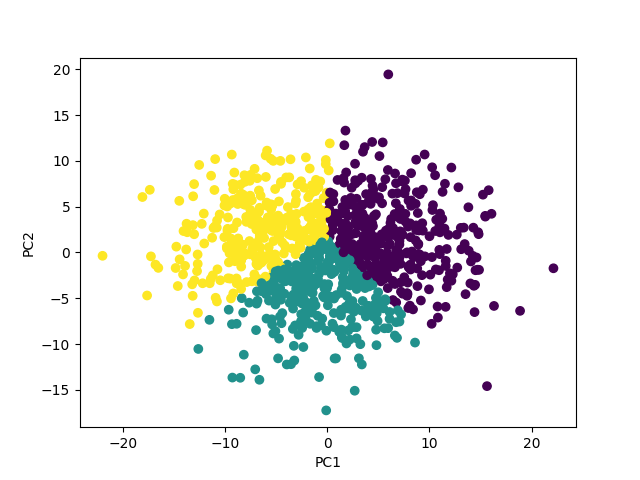
\includegraphics[width=\linewidth]{../results/plots/scatter_carino_kmeans}
         \caption{5 cluster}
     \end{subfigure}
     \begin{subfigure}[b]{0.49\linewidth}
         \centering
         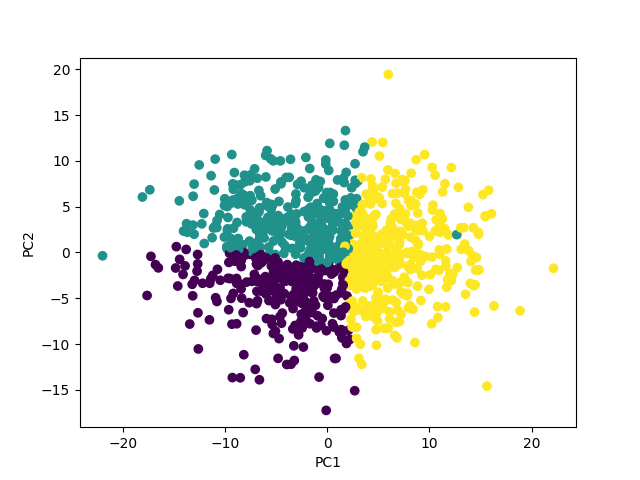
\includegraphics[width=\linewidth]{../results/plots/scatter_carino}
         \caption{7 cluster}
     \end{subfigure}
     \caption{Scatterplot dei dati clusterizzati}
     \label{fig:2}
    \end{figure}

    \subsection{Dataset sintetici}


    \subsection{Dataset real-world}
    In questa sezione analizziamo gli esperimenti svolti su dataset real-world. Il primo dataset considerato è Heart Disease. Contiene

    Gli esperimenti sono stati eseguiti su sottoinsiemi di tali dataset con caratteristiche diverse. Sono stati infatti variati parametri quali numero di esempi, numero di features e numero di cluster. In tutti i casi è stato impostato un time-limit per la versione MIQP, in modo da ottenere risultati significativi in tempi ragionevoli.\\
    La Figura \ref{fig:7} mostra i risultati ottenuti al variare del numero di elementi del dataset, fissando il numero di features $N=4$ e il numero di cluster $K=3$. Come spiegato in (Lapucci et), la versione MIQP dovrebbe essere particolarmente sensibile al numero di variabili binarie del problema; poiché il numero di elementi è fatto variare in $n=10,20,...,60$, il numero di variabili in gioco ha un un minimo di 30 e un massimo di 180.\\
    \begin{figure}[H]
     \centering
     \begin{subfigure}[t]{0.49\linewidth}
         \centering
         \includegraphics[width=\linewidth]{../results/plots/loss_size_real}
         \caption{Valore finale della funzione obiettivo}
     \end{subfigure}
     \hfill
     \begin{subfigure}[t]{0.49\linewidth}
         \centering
         \includegraphics[width=\linewidth]{../results/plots/runtime_size_real}
         \caption{Tempo di esecuzione: tempo impiegato da Kmeans per raggiungere la soluzione sub-ottimale (arancio); tempo impiegato da MIQP per raggiungere la migliore soluzione trovata (verde); tempo impiegato da MIQP per raggiungere una soluzione migliore di Kmeans (rosso)}
     \end{subfigure}
        \label{fig:7}
        \caption{Performance al variare del numero di elementi}
     \end{figure}
    Risulta evidente che all'aumentare del numero di esempi nel dataset, la versione MIQP impiega sempre più tempo per raggiungere la soluzione ottima. In particolare, per dataset di dimensioni maggiori di 40 elementi, la versione MIQP non riesce a raggiungere la soluzione sub-ottima ottenuta con K-means in tempi ragionevoli.\\
    Allo stesso modo è aspettabile che anche il numero di cluster scelto possa influenzare le performance dell'algoritmo. In Figura \ref{fig:8} sono mostrati i risultati ottenuti fissando il numero di elementi $n=30$ e il numero di features $N=4$. In particolare il numero di centroidi con cui viene inizializzato l'algoritmo sembra essere un fattore ancora più significativo per le performance della versione MIQP.
    \begin{figure}[H]
     \centering
     \begin{subfigure}[t]{0.49\linewidth}
         \centering
         \includegraphics[width=\linewidth]{../results/plots/loss_centers_real}
         \caption{Valore finale della funzione obiettivo}
     \end{subfigure}
     \hfill
     \begin{subfigure}[t]{0.49\linewidth}
         \centering
         \includegraphics[width=\linewidth]{../results/plots/runtime_centers_real}
         \caption{Tempo di esecuzione: tempo impiegato da Kmeans per raggiungere la soluzione sub-ottimale (arancio); tempo impiegato da MIQP per raggiungere la migliore soluzione trovata (verde); tempo impiegato da MIQP per raggiungere una soluzione migliore di Kmeans (rosso)}
     \end{subfigure}
        \label{fig:8}
        \caption{Performance al variare del numero di cluster}
     \end{figure}
    Diversamente, il numero di feature non varia la quantità di variabili di associazione tra esempi e cluster, dunque dovrebbe avere un'influenza minore sulla differenza di performance. Si può infatti osservare in Figura \ref{fig:9} che, con tutti i valori di $N$ testati, la variante MIQP riesce a raggiungere la soluzione sub-ottima ottenuta con K-means in tempi ragionevoli. Inoltre non è visibile una netta correlazione tra il numero di feature e il tempo di esecuzione della versione MIQP.
    \begin{figure}[H]
     \centering
     \begin{subfigure}[t]{0.49\linewidth}
         \centering
         \includegraphics[width=\linewidth]{../results/plots/loss_features_real}
         \caption{Valore finale della funzione obiettivo}
     \end{subfigure}
     \hfill
     \begin{subfigure}[t]{0.49\linewidth}
         \centering
         \includegraphics[width=\linewidth]{../results/plots/runtime_features_real}
         \caption{Tempo di esecuzione: tempo impiegato da Kmeans per raggiungere la soluzione sub-ottimale (arancio); tempo impiegato da MIQP per raggiungere la migliore soluzione trovata (verde); tempo impiegato da MIQP per raggiungere una soluzione migliore di Kmeans (rosso)}
     \end{subfigure}
        \label{fig:9}
        \caption{Performance al variare del numero di cluster}
     \end{figure}

\end{document}
